\chapter{Projeto de implementação}
\label{cap:projetoimplementacao}

Neste capítulo será apresentados os serviços considerados mais críticos da empresa. Posteriormente, será proposta uma solução de implementação 
de alta disponibilidade. Essa solução será detalhada na Seção \ref{section:propostasolucao}, e será baseada na utilização de virtualização e
\textit{softwares} de código aberto. 

\section{Levantamento dos serviços críticos}
\label{section:servcrit}

No capítulo anterior foram detalhados todos os serviços que estão disponíveis na empresa. Sendo assim, nesta seção será feito uma análise desses
serviços, destacando os serviços considerados mais críticos para a empresa. Para a seleção dos serviços críticos foram adotados os seguintes
critérios:
\begin{itemize}
 \item A quantidade de clientes ou funcionários que utilizam o serviço: esse é o item mais relevante, pois impacta diretamente no faturamento
 da empresa. De fato, se um cliente ficar sem acesso à Internet, o cliente terá um desconto proporcional, ao tempo que ficou sem 
 acesso; 
 \item O número de requisições em um determinado tempo: esse número é importante, uma vez que, indicam a quantidade de usuários que dependem do 
 serviço. São exemplos dessa medida a quantidade de acessos por minuto em um servidor de hospedagens de sites e a quantidade de requisições 
 \ac{DNS} em um servidor recursivo;
 \item O volume de elementos do serviço: essa medida demonstra a abrangência do serviço, ou seja, quantos clientes são dependentes deste. 
 Como exemplo de elementos pode-se citar a quantidade de contas de \textit{e-mail} em um servidor de \textit{e-mail} e a quantidade de 
 equipamentos monitorados por um servidor de monitoramento. 
 %Esse critério é importante pois com ele pode-se comparar diferentes serviços possibilitando perceber o grau de relevância que cada um possui;
 \item O número de conexões \ac{TCP} \cite{tanenbaum2011} ou o número de requisições \ac{UDP} \cite{tanenbaum2011}: essa medida demonstra a 
 quantidade de acessos simultâneos que um serviço possui. 
 %Esse critério, como o anterior, também permite comparar diferentes serviços para ter a possibilidade de ordená-los de acordo com sua relevância, por isso o torna importante para esta análise.
\end{itemize}

Nas próximas seções serão descritos os serviços considerados críticos.

\subsection{\ac{DNS} recursivo primário}
\label{section:dnsrecprim}

Esse serviço foi classificado como o mais importante pois possui um impacto direto nos clientes do provedor. Esse é o único serviço que todos 
os clientes e funcionários utilizam. O objetivo de um provedor é fornecer uma navegação de qualidade aos seus clientes, sendo assim, o \ac{DNS} 
é fundamental para essa navegação, uma vez que é usado por todos os clientes, que é aproximadamente 9000. Outro importante critério que pode ser 
aplicado ao \ac{DNS} recursivo é o número de requisições por segundo. Como pode ser observado na Figura \ref{fig:dns_udp} (a) esse serviço
possui aproximadamente 1150 requisições por segundo. De acordo com a Figura \ref{fig:dns_udp} (b), que compara os principais servidores da 
empresa através de requisições \ac{UDP}, onde pode-se observar que o servidor \textit{Passata} possui um grande número de requisições 
\ac{UDP}\footnote[1]{Esse número de requisições \ac{UDP} são elevadas devido ao fato do serviço \ac{DNS} gerá-las.}.

\begin{figure}[h!]
 \centering
 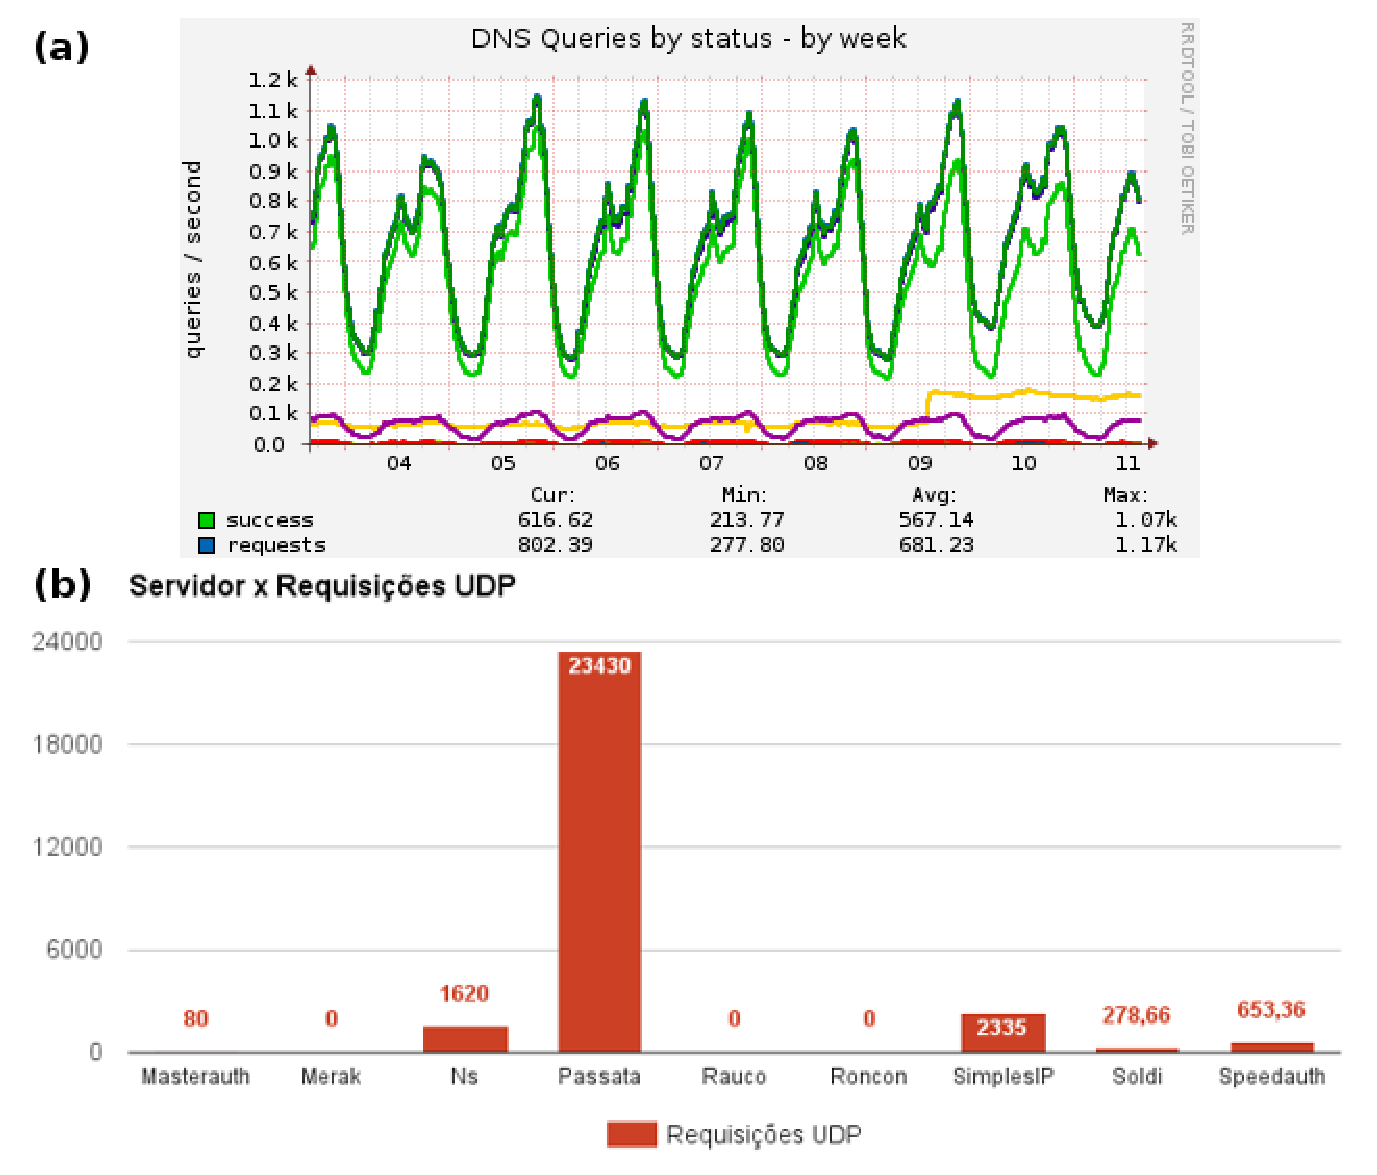
\includegraphics[width=400px]{img/dns_udp.eps}
 \caption{Gráfico de requisições DNS (a) e comparação de requisições UDP entre os principais servidores (b).}
 \label{fig:dns_udp}
\end{figure}

\subsection{Radius}
\label{section:radius}

Esse serviço é importante pois é o responsável pela autenticação de todos os clientes do provedor. Caso esse serviço fique indisponível, 
os clientes não conseguirão estabelecer conexão para sua navegação. Os servidores \textit{Masterauth} e \textit{Speedauth} fornecem o serviço de
\textit{Radius}, sendo que recebem, em média, 1,6 requisições de autenticação por segundo, como pode ser observado na Figura 
\ref{fig:freeradius_auth} (a) e na \ref{fig:freeradius_auth} (b). Caso esses servidores ficarem indisponíveis aproximadamente 1,6 clientes 
não conseguirão efetuar a autenticação para iniciar a sua navegação. Além disso, esses servidores armazenam alguns dados relacionados à conexão 
dos clientes, como por exemplo o endereço de \ac{IP} que é utilizado por um cliente em um determinado período, o tráfego de dados da conexão, 
o tempo da conexão de cada cliente, o endereço \ac{MAC} dos equipamentos dos clientes, entre outros. Essas operações resultam em média 23 
requisições por segundo. %, como pode ser observado na Figura \ref{fig:speedauth_acct_week} e \ref{fig:masterauth_acct_week};
Outro critério que é relevante para esses servidores é o volume de elementos do serviço, que neste caso, representa a quantidade de \textit{logins} 
de autenticação dos clientes. Como pode ser obervado na Figura \ref{fig:elementos_tcp} (a), os servidores \textit{Masterauth} e \textit{Speedauth}
estão entre os que apresentam o maior número de elementos. Além disso, existe um destaque desses servidores no número de conexões \ac{TCP}, como 
pode ser observado na Figura \ref{fig:elementos_tcp} (b).

\begin{figure}[h!]
 \centering
 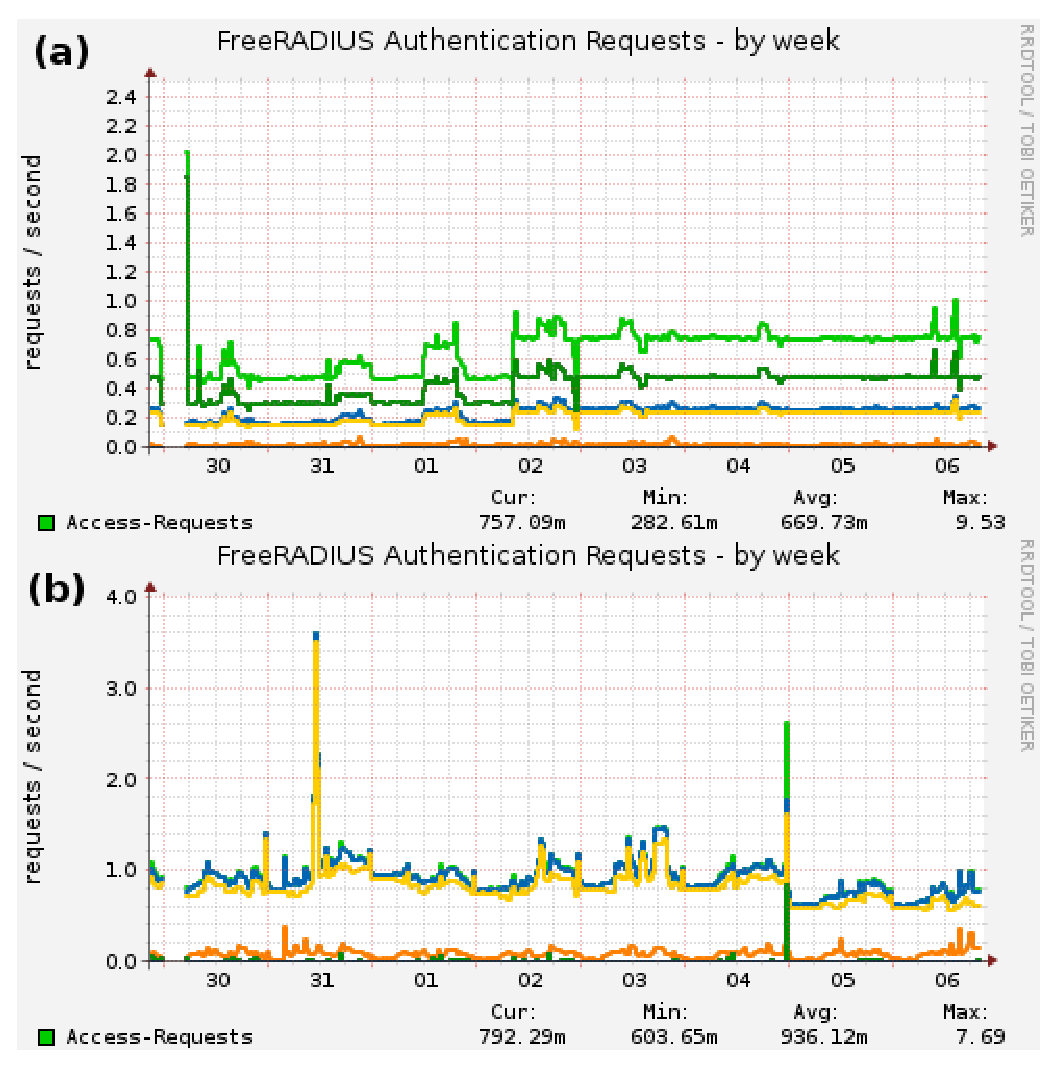
\includegraphics[width=350px]{img/freeradius_auth.eps}
 \caption{Gráfico de requisições de autenticação do servidor Masterauth (a) e Speedauth (b).}
 \label{fig:freeradius_auth}
\end{figure}

\begin{figure}[h!]
 \centering
 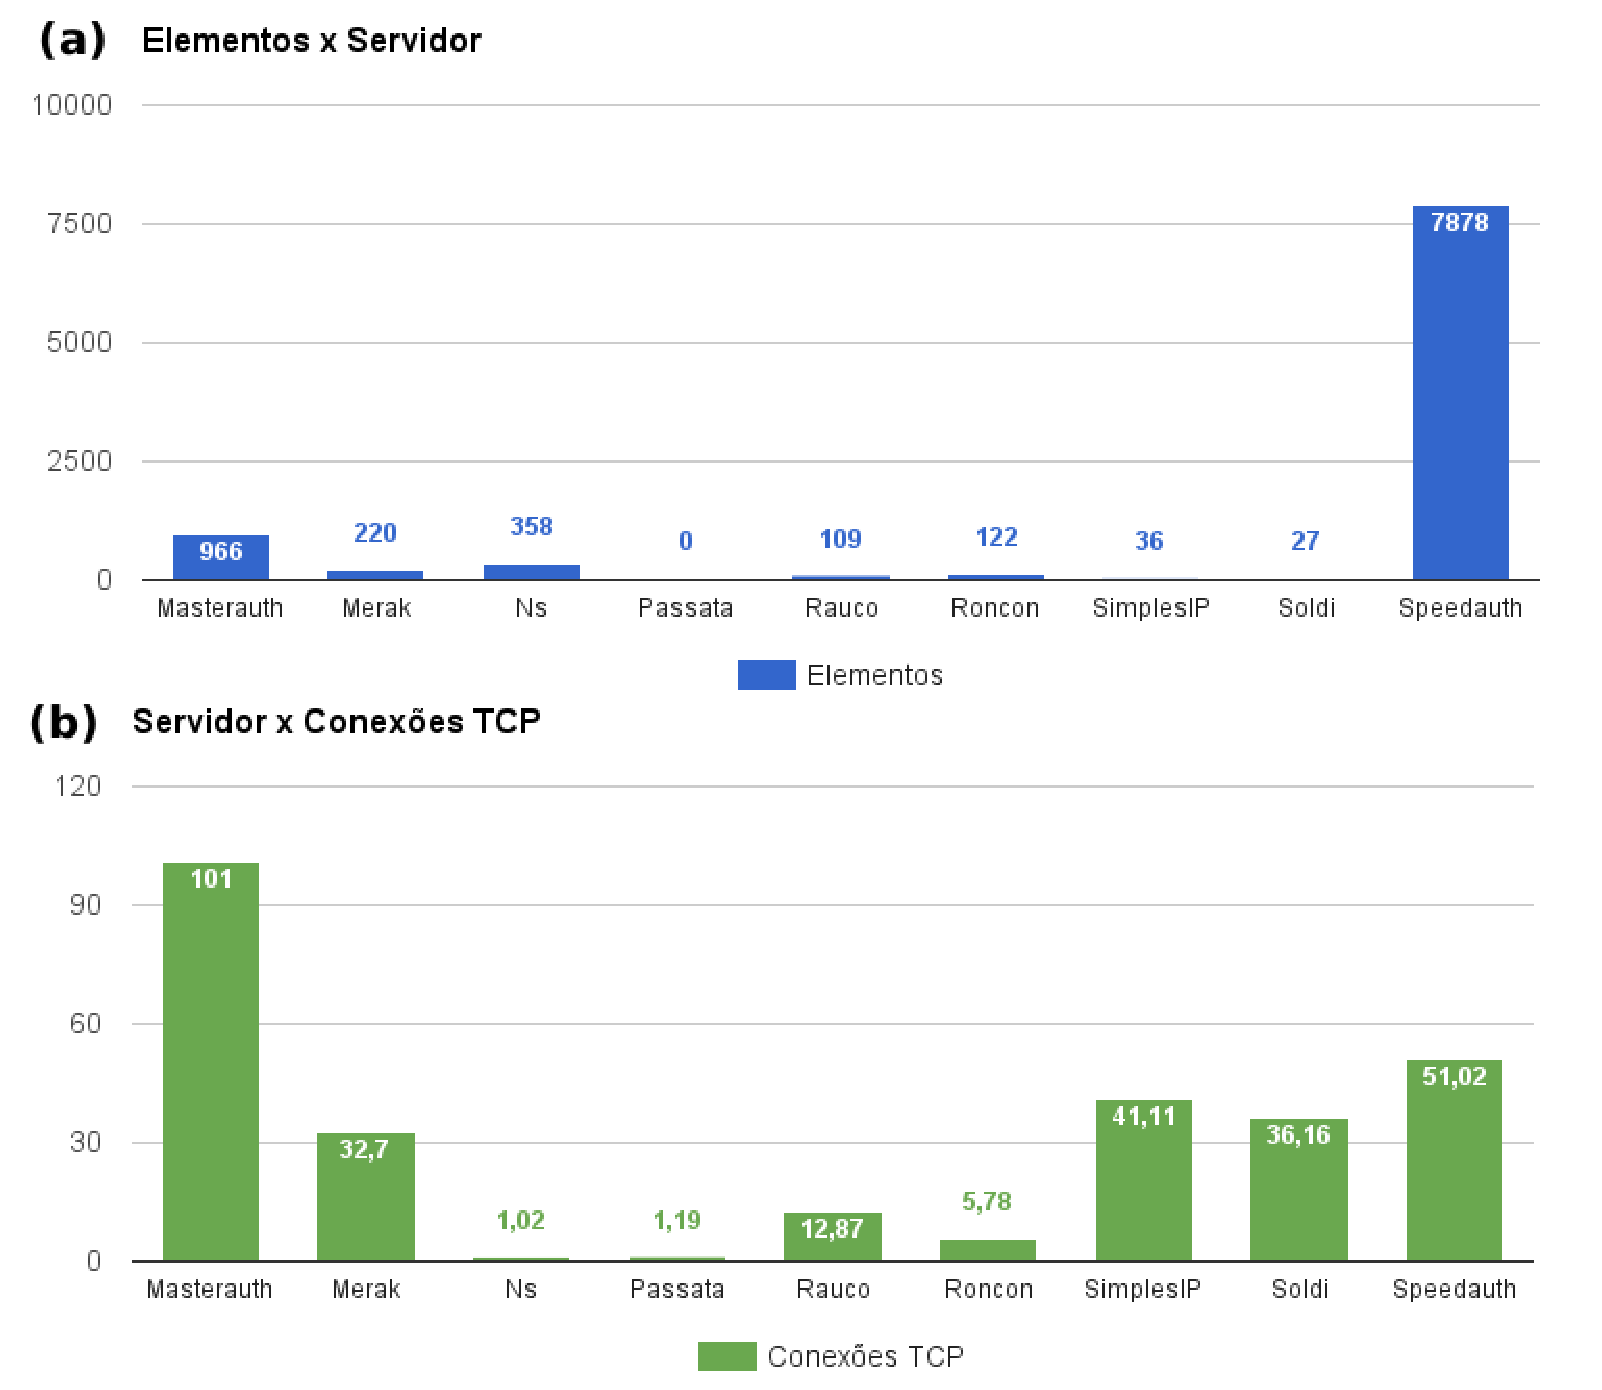
\includegraphics[width=400px]{img/elementos_tcp.eps}
 \caption{Gráfico de comparação de elementos (a) e de conexões TCP (b) entre os principais servidores.}
 \label{fig:elementos_tcp}
\end{figure}

\subsection{Sistemas da empresa e do provedor}
\label{section:sistemas}

O sistema do provedor é responsável pela maior parte das operações do provedor. De fato, esse sistema é responsável pela emissão de boletos, 
atendimento de clientes, comunicação interna da empresa, vendas, ativações de novos clientes, entre outros. Esse sistema não tem um impacto 
direto para os clientes, porém é fundamental para o funcionamento da empresa e do provedor. Caso haja uma indisponibilidade desses sistemas 
a maior parte dos funcionários ficarão impossibilitados de trabalhar, sendo que a empresa possui no total 65 funcionários.
%, sendo que são aproximadamente 35 funcionários simultâneos (de acordo com a Figura \ref{fig:ejabberd_week}), isso poderia gerar um prejuizo elevado para a empresa e o provedor. 
Esse sistema é executado no servidor \textit{Soldi} que recebe aproximadamente 3 requisições \textit{HTTP} \cite{tanenbaum2011} por segundo 
número de requisições por segundo, como pode ser observado na Figura \ref{fig:soldi_week}. Além disso, a empresa mantém outros 27 sistemas, 
de outros clientes, nesse mesmo servidor. 
Outro critério que aplica-se a esse serviço é o número de conexões \ac{TCP}, onde pode-se observar que o servidor \textit{Soldi} está 
entre os mais relevantes, como pode ser observado na Figura \ref{fig:elementos_tcp} (b). 

%\begin{figure}[h!]
% \centering
% 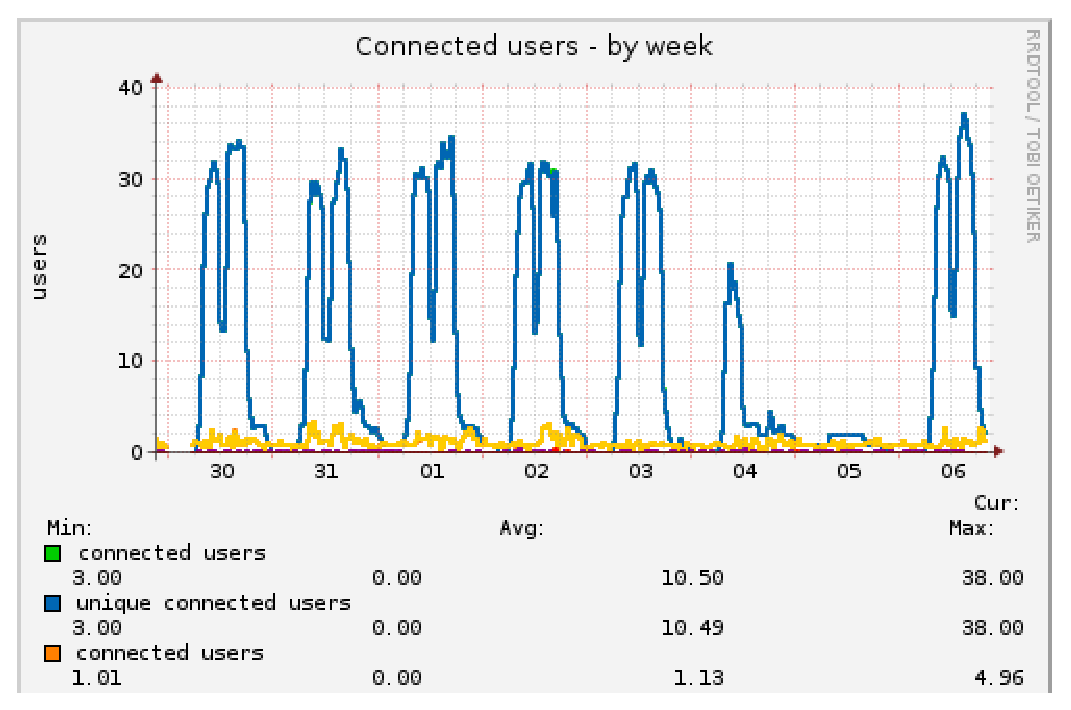
\includegraphics[width=310px]{img/ejabberd_week.eps}
% \caption{Gráfico usuários simultâneos de sistema.}
% \label{fig:ejabberd_week}
%\end{figure}

\begin{figure}[h!]
 \centering
 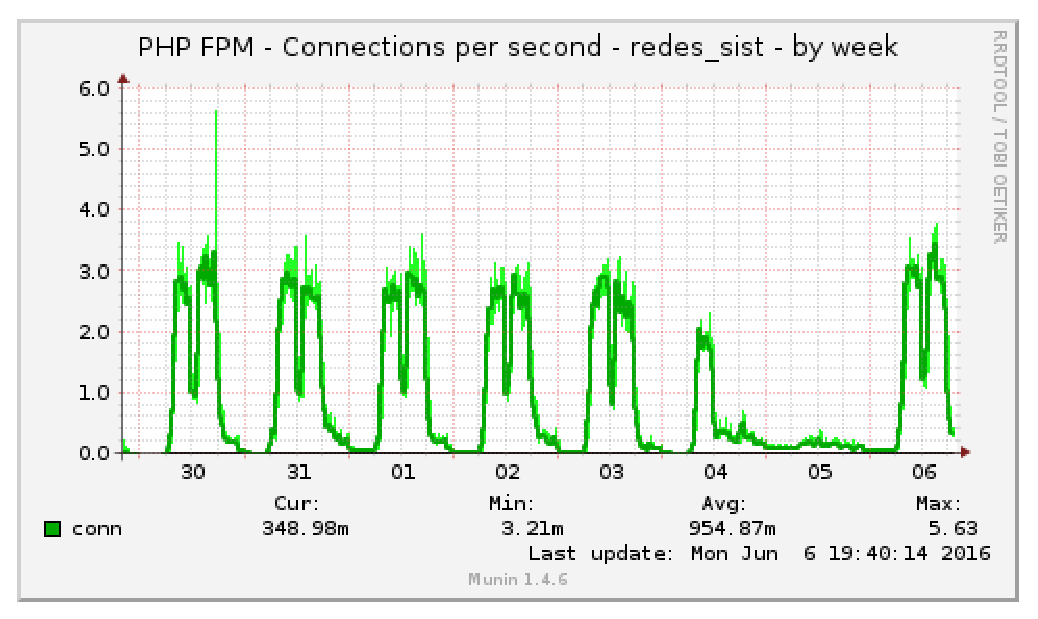
\includegraphics[width=310px]{img/soldi_week.eps}
 \caption{Gráfico de requisições por segundo do maior sistema.}
 \label{fig:soldi_week}
\end{figure}

\subsection{Telefonia}
\label{section:telefonia}

Esse serviço tem relevância para a empresa e para o provedor, pois permite a comunicação entre os clientes e os funcionários, ou seja, o 
servidor \textit{SimplesIP} é responsável por garantir o atendimento a clientes para fins de suporte técnico, comunicação interna entre 
funcionários, comunicação com técnicos externos, vendas, cobranças a clientes, entre outros. Para quantificar, no mês de maio de 2016 a empresa 
recebeu 15922 ligações, com duração total de 67 horas e 40 minutos. Além disso, no mesmo mês foram efetuadas 674 ligações entre funcionários. 
O gráfico da Figura \ref{fig:simplesip_week} mostra a quantidade de canais ativos no servidor de telefonia. Observa-se nesta figura que ocorre 
de 20 a 30 ligações simultâneas durante o horário comercial, que é das 08:00 às 12:00 e das 13:00 às 18:00. Além disso, na Figura 
\ref{fig:dns_udp} (b) observa-se o número de requisições \ac{UDP} recebidas\footnote[1]{Esse número de requisições \ac{UDP} deve-se ao fato
da telefonia utilizar o protocolo \ac{UDP} para transmissão de voz.}.

\begin{figure}[h!]
 \centering
 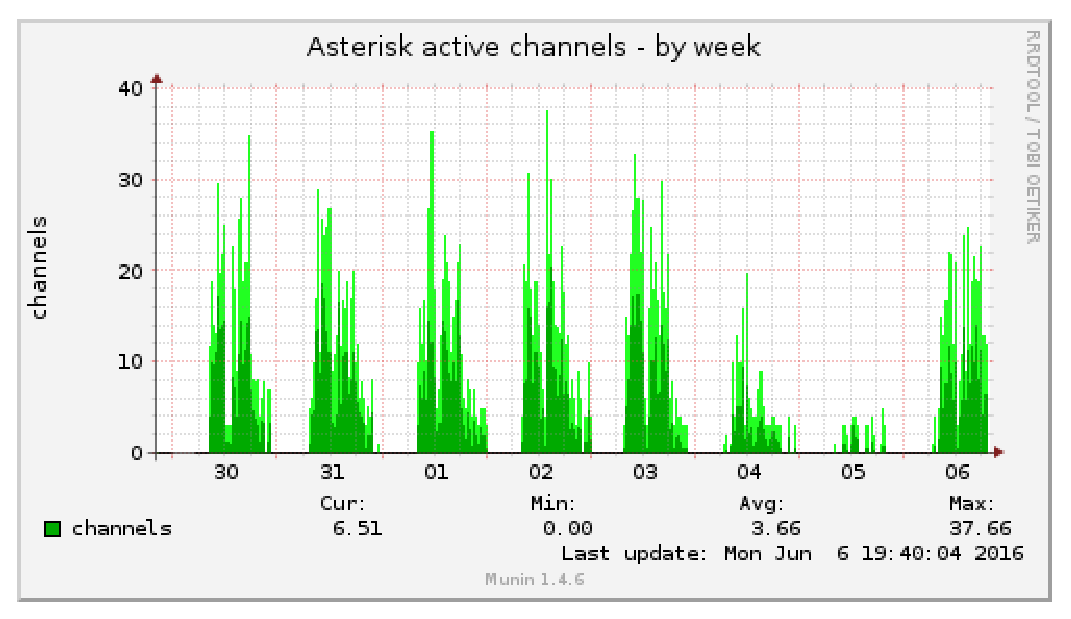
\includegraphics[width=310px]{img/simplesip_week.eps}
 \caption{Gráfico de requisições por segundo do maior sistema.}
 \label{fig:simplesip_week}
\end{figure}

\subsection{Máquinas com serviços críticos}
\label{section:maqservcrit}

Desta forma, verifica-se que os servidores a serem incluídos no ambiente de alta disponibilidade são:
\begin{itemize}
 \item \textit{Passata}
 \item \textit{Speedauth}
 \item \textit{Masterauth}
 \item \textit{Soldi}
 \item \textit{SimplesIP}
\end{itemize}

Incluir tabela com disponibilidade atual ??


\section{Proposta de solução}
\label{section:propostasolucao}

Para implementar esta solução será necessário dois servidores físicos, sendo que a configuração de cada servidor deverá ser de 
11 \textit{cores} de processamento, 12 GB de memória \ac{RAM} e 156 GB de disco. Essa configuração foi calculada a partir da soma dos recursos 
atuais das máquinas virtuais que possuem os serviços críticos, que foram apresentadas na Seção \ref{section:servcrit}.
Com essa solução, caso ocorra alguma falha em um servidor, as máquinas virtuais serão transferidas para o outro servidor.
Inicialmente, para obter-se esse \textit{hardware}, que é necessário para implementação, será feito uma reorganização nas máquinas virtuais.

As ferramentas necessárias para a implementação podem ser divididas em dois grupos, ferramentas de replicação de dados de alta disponibilidade
(Seção \ref{section:toolrepl}) e ferramentas para o monitoramento e a tranferências das máquinas virtuais entre os servidores 
(Seção \ref{section:toolcluster}).

\subsection{Ferramentas de replicação de dados}
\label{section:toolrepl}

Replicação de dados pode ser realizada de diferentes formas, que podem ser a nível de aplicação ou até mesmo a nível de \textit{hardware}.
Dependendo do objetivo e da aplicação pode-se usar ferramentas como, por exemplo, o \textit{rsync} \cite{rsync}, que faz o sincronismo de dados 
copiando os dados de um servidor de origem para um de destino. Essa não pode ser usada neste contexto pois ela não faz a sincronização em tempo
real. Outra forma de replicação em \textit{hardware} é a utilização de discos em \ac{RAID} \cite{raid}. Essa solução é eficaz para garantir que 
o sistema não fique indisponível em caso de falha de discos\footnote{Lembrando que essa solução é utilizada no ambiente atual para aumentar a 
disponibilidade dos servidores.}, porém não garante a disponibilidade quando \textit{software} ou algum outro componente de \textit{hardware} 
falhar \cite{zaminhani2008}.

A solução de replicação a ser adotada consiste em um espelhamento de dados através da rede. Essa solução permite a cópia dos dados de um servidor
para um servidor remoto em tempo real. A seguintes ferramentas de replicação de dados foram encontradas:
\begin{itemize}
 \item \ac{DRBD} \cite{drbd}
 \item \textit{GlusterFS} \cite{glusterfs}
 \item \textit{Ceph RBD} \cite{cephrbd}
 \item \textit{Rsync} \cite{rsync}
\end{itemize}
% Swift open stack
% https://wiki.freebsd.org/HAST

A Tabela \ref{tab:replicacao} compara as ferramentas citadas anteriormente. Nesta tabela, pode-se perceber que o \textit{Rsync} não pode ser
utilizado pois não faz replicação em tempo real. Já o \textit{GlusterFS} pode ser utilizado neste trabalho, porém sua principal característica, 
que é a escalabilidade, ou seja, facilidade em aumentar os nós do \textit{cluster}, não será útil para esta implementação.
Além disso ele faz a replicação a nível de arquivo, assim pode-se obter um desempenho inferior.
E por fim, o \textit{Ceph RBD} necessita de um \textit{hardware} adicional para monitorar e administrar, além disso, ele executa o 
\textit{storage} (Ceph ODS) em um \textit{hardware} separado dos nós que fazem o processamento (clientes MDS).

\begin{table}[h!]
\caption{Comparação ferramentas de replicação de dados.}
\label{tab:replicacao}
\begin{center}
\begin{tabular}{|l|p{2.7cm}|p{2.7cm}|p{2.7cm}|p{2cm}|}\hline
Características & DRBD & GlusterFS & Ceph RBD & Rsync\\\hline
Master/Slave & Sim & Sim & Não & Não \\\hline
Replicação em tempo real & Sim & Sim & Sim & Não \\\hline
Nível de replicação & Bloco & Arquivo & Bloco & Arquivo \\\hline
Número máximo de nós & 16 & 64 & Ilimitado & Ilimitado \\\hline
Plataformas & Suse, Debian, CentOS, Red Hat, Ubuntu & Debian, CentOS, Red Hat, Fedora, Ubuntu & CentOS, Red Hat, Debian, Fedora, Ubuntu & Linux \\\hline
Integração com virtualização & Sim & Sim & Sim & Não \\\hline
\end{tabular}
\end{center}
\end{table}

%https://www.reddit.com/r/linux/comments/1qwarp/drbd_vs_glusterfs/
% glusterfs mais escalavel, simples de administrar
% drbd melhor eficiencia(acredito) nivel de bloco, confiavel(10 anos develop)

% drbd: 2 nodes na versão 8 e 16 nodes por stacking / 16 nodes na versão 9

% drbd dispositivo primário e secundário zaminhani2008
% Segundo (ELLENBERG, 2007), a partir da versão 8 do DRBD é possível que,
%dependendo da aplicação, a execução ocorra em todos os nós do cluster
%simultaneamente (Ativo/Ativo). Para tornar isso possível é necessária a
%utilização de um sistema de arquivos exclusivo para cluster, como o OCFS2 6 e o
%GFS 7 por exemplo. Como a abordagem deste trabalho é cluster de alta
%disponibilidade, a utilização do DRBD no modo Ativo/Ativo não será discutida.

% glusterfs https://raobharata.wordpress.com/2012/10/29/qemu-glusterfs-native-integration/
% melhor performace com disco utilizando protocolo gluster file=gluster://path/to

% ceph http://docs.ceph.com/docs/master/start/intro/
% necessita um hardware especifico para monitor, outra para dados e metadata

A ferramenta escolhida para replicação de dados na solução de alta disponibilidade desse trabalho foi o \ac{DRBD}, pois permite a configuração 
\textit{master-slave}, suporte replicação de imagens de máquinas virtuais e faz replicação a nível de bloco, o que possibilita maior segurança
dos dados e um melhor desempenho.
Essa ferramenta é de código aberto, e permite a replicação de dados de um dispositivo. Os dispositivos \ac{DRBD}, possuem os estados primário 
e secundário. Entretanto, apenas um nó do \textit{cluster} pode ser o nó primário, sendo que esse nó é o único que terá permissão para acessar 
o dispositivo, ou seja, somente ele poderá fazer operações de leitura e escrita. Na Figura \ref{fig:drbd_basic} tem-se dois servidores com seus 
respectivos discos, \textit{hda1} e \textit{hda3}, formando um \textit{cluster}, sendo que esses discos estão sincronizados através da rede. 
Com isso, todas as operações de escritas feitas no nó primário serão replicadas para o disco do nó secundário \cite{zaminhani2008}.

\begin{figure}[h!]
 \centering
 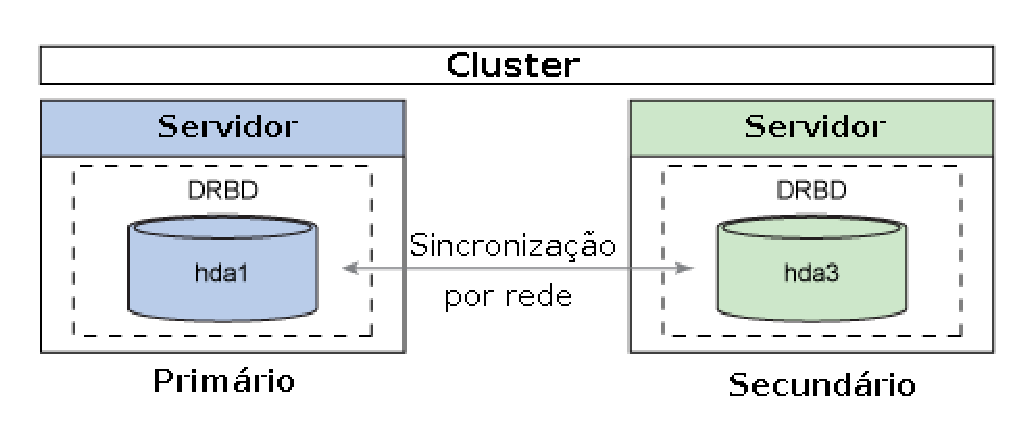
\includegraphics[width=300px]{img/drbd_basic.eps}
 \caption{Modelo DRBD}
 Fonte: \citet{jones2010}
 \label{fig:drbd_basic}
\end{figure}

\subsection{Ferramentas de gerenciamento de cluster}
\label{section:toolcluster}

Para ser possível implementar uma solução de alta disponibilidade é necessário organizar os servidores em uma estrutura de \textit{cluster}.
%uma ferramenta que monitora os recursos, fazendo a detecção e recuperação do serviço utilizando mensagens entre os servidores, que é denominada como um \textit{cluster} \cite{perkov2011}. 
Pode-se definir \textit{cluster} como um grupo de computadores interligador por rede com o objetivo de aumentar o desempenho ou disponibilidade
de um serviço \cite{freitas2005}.

Além disso, é necessário a utilização de ferramentas para facilitar o gerenciamento desse \textit{cluster}. Essas permitem detectar falhas em um 
nó ou a nível de recursos, ou seja, essas podem detectar falhas de \textit{hardware} e falhas de serviços. Essas ferramentas são conhecidas 
como \ac{CRM}, cuja função é fazer a gerência de recursos de um \textit{cluster}.

A Tabela \ref{tab:clusterger} compara as ferramentas de acordo com algumas características. Pode-se observar que a ferramenta \textit{Pacemaker}
pode ser configurada para fazer monitoramento e recuperação tanto a nível de nó quanto a nível de recurso.
O \textit{Ganeti} é um gerenciador de \textit{cluster} de virtualização, ...
O \textit{Ceph} é uma ferramenta unificada de armazenamento de dados distribuída, ...
É possível também implementar essa solução com a ferramenta \textit{Heartbeat}, porém, desta forma seria necessário criar um conjunto de \textit{scripts} 
para fazer a migração das máquinas virtuais, o que dificultaria a implementação.
O \textit{Heartbeat} é um subprojeto do \textit{Linux-HA} \cite{linuxha}, que desenvolve aplicações para soluções de alta disponibilidade.
Esse subprojeto é uma aplicação que envia pacotes \textit{keepalive \ac{UDP}} através da rede para outras instâncias do \textit{Heartbeat}, para
informar se ele está ativo \cite{reis2009}.

\begin{table}[h!]
\caption{Comparação ferramentas de gerenciamento de cluster.}
\label{tab:clusterger}
\begin{center}
\begin{tabular}{|p{3.5cm}|p{2.7cm}|p{2.7cm}|p{2.7cm}|p{2cm}|}\hline
Características & Pacemaker & Ceph & Ganeti & Heartbeat \\\hline
Sincronismo de configuração entre os nós & Sim &  & Não & Não \\\hline
Failover e failback & Sim & Sim & Sim & Não \\\hline
Nível de detecção e recuperação & Nó e recurso &  & Nó e máquina virtual & Nó \\\hline
Plataformas & Red Hat, CentOS, Fedora, Suse, Debian, Ubuntu & CentOS, Debian, Fedora, Red Hat, Ubuntu & Linux & Red Hat, CentOS, Fedora, Suse, Debian, Ubuntu \\\hline
Integração com virtualização & Sim & Sim & Sim & Sim \\\hline
\end{tabular}
\end{center}
\end{table}

% ganeti pode ser usado com ceph rdb (RADOS Cluster), ou drbd

O \ac{CRM} escolhido para gerenciar o ambiente que será criado neste trabalho foi o \textit{Pacemaker}, pois é uma ferramenta flexível ... 
e de código aberto. 

O \textit{Pacemaker} \cite{pacemaker} pode ser definido como uma ferramenta de recuperação de falhas a nível de serviço \cite{perkov2011}. 
Essa ferramenta é um projeto de código aberto mantido pela \cite{clusterlabs}, e teve origem com a necessidade de aperfeiçoar o gerenciador 
de recursos, que possuía algumas limitações, da ferramenta \textit{Heartbeat} \cite{heartbeat}. Esse \ac{CRM} funciona juntamente com ferramentas
que fazem troca de mensagens entre os nós do \textit{cluster} e ferramentas que fazem a afiliação, ou seja, fazem o processo de registro dos
nós, de \textit{failover} e de bloqueios distribuídos, quando utilizado sistema de arquivos distribuídos. 
Definir failover ??
\cite{bassan2008} pag 20
%\cite{borne} pag 11
%\cite{costa2009} pag 39

As ferramentas que podem ser integradas com o \textit{Pacemaker} são:
\begin{itemize}
 \item \textit{Corosync}: é responsável pelo processo de registro dos nós, de \textit{failover} e de bloqueios distribuídos (utilizados para 
 implementar cLVM, GFS/GFS2, e OCFS2), entre outros. Essa ferramenta derivou do projeto \textit{OpenAIS};
 \item \textit{Heartbeat}: é um mecanismo que faz envio de mensagens entre os nós do \textit{cluster} com objetivo de notificar esse 
 \textit{cluster} quando houver alguma alteração de estado dos recursos ou dos nós \cite{clusterlabs}.
\end{itemize}
% outras ferramentas cMAN e Apache Qpid

Na Figura \ref{fig:pacemaker_tools} pode-se observar a camada inferior com os nós do \textit{cluster}, logo acima as ferramentas de envio de 
mensagens, acima delas fica o \textit{Pacemaker}, e por fim o \textit{DRBD} e os serviços dos servidor.

\begin{figure}[h!]
 \centering
 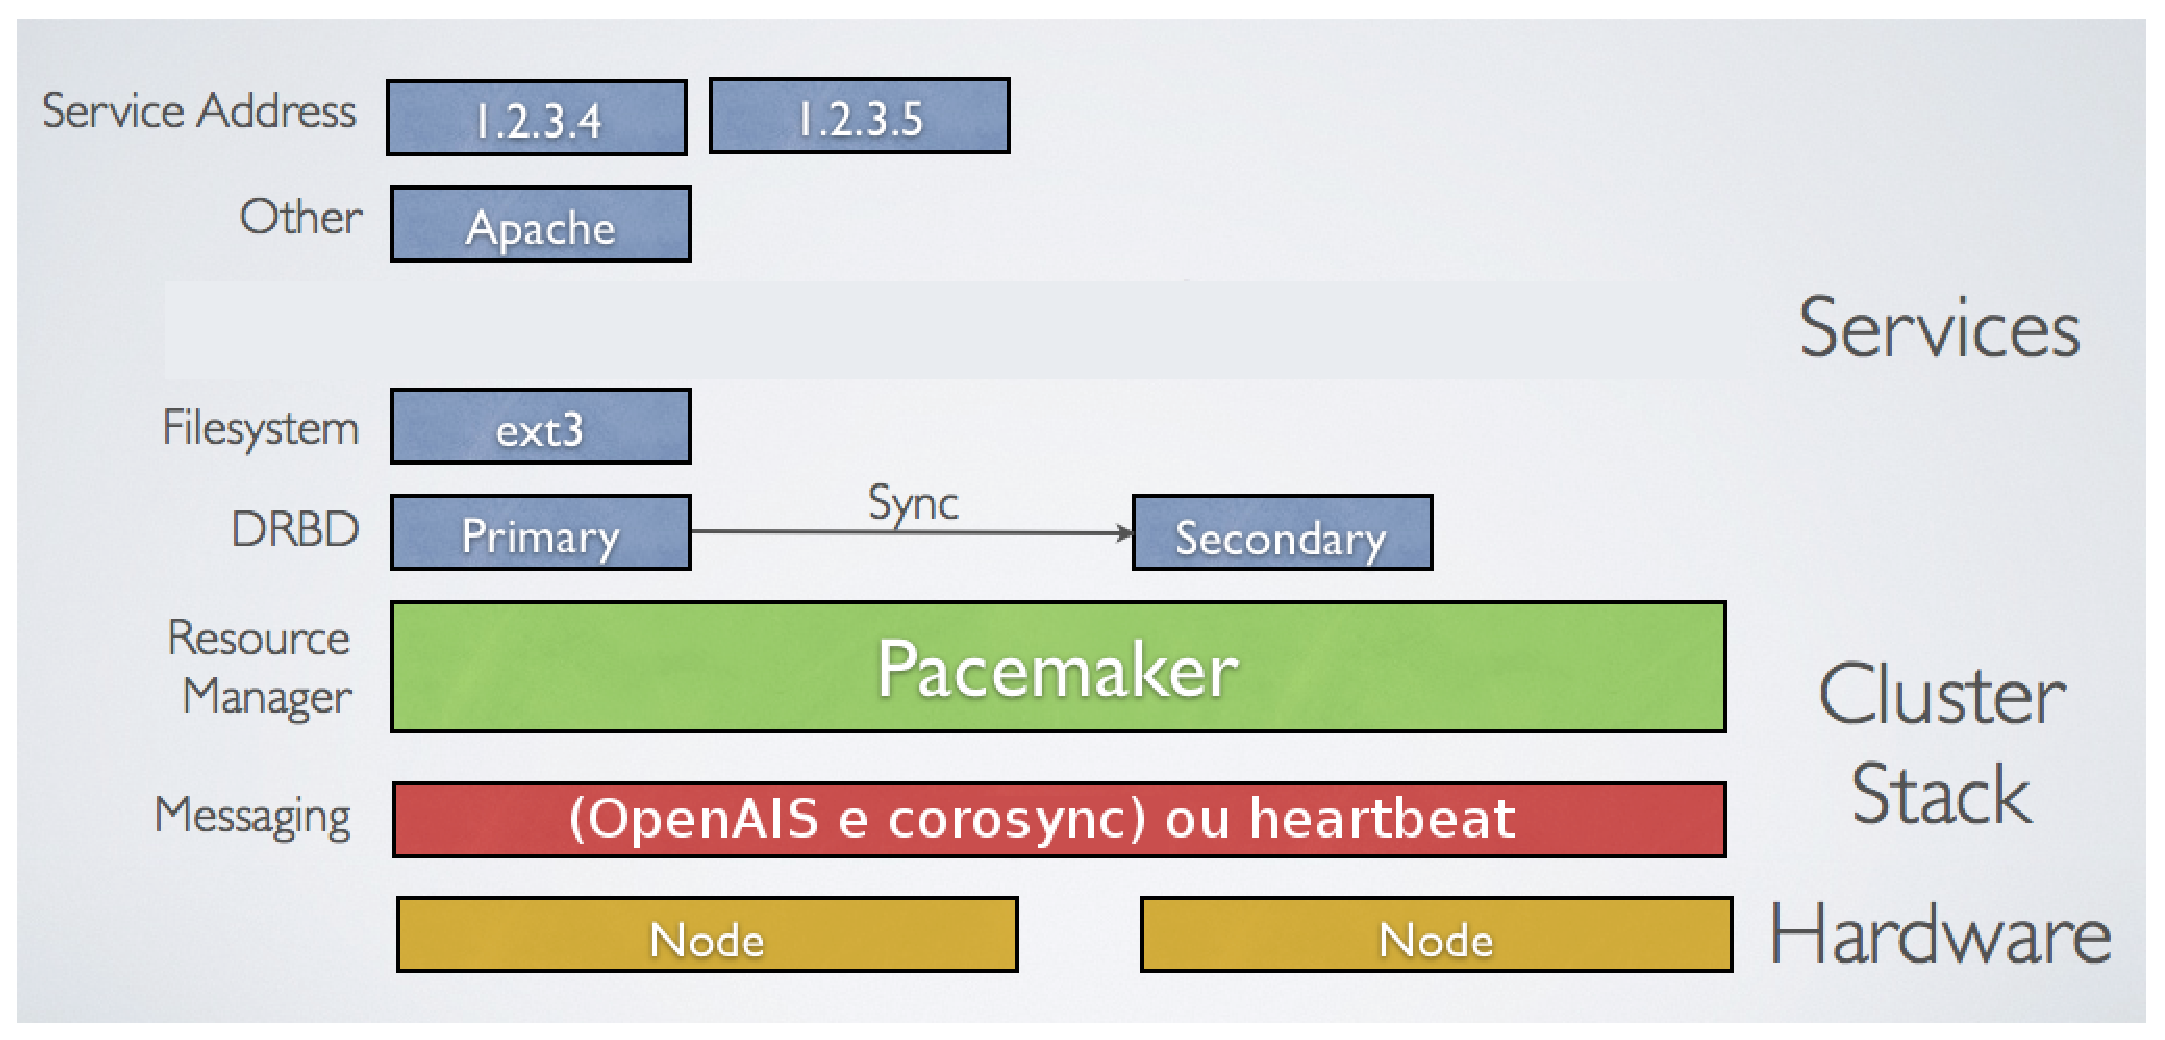
\includegraphics[width=280px]{img/pacemaker_tools.eps}
 \caption{Pacemaker estrutura}
 Fonte: \citet{pacemaker}
 \label{fig:pacemaker_tools}
\end{figure}

% Como citado anteriormente, o \textit{Pacemaker} funciona juntamente com outras ferramentas. Sendo assim, a sua arquitetura pode ser 
% dividida em três partes:
% \begin{itemize}
%  \item Componentes não-cluster:
%  \item Gerência de recursos: 
%  \item Camada de troca de mensagens:
% \end{itemize}

O \ac{CRM} \textit{Pacemaker} possui algumas funções principais que estão listadas abaixo:
\begin{itemize}
 \item Inicia e para serviços dos nós do \textit{cluster}, esses serviços podem ser desde um servidor \textit{web} até uma interface de rede, 
 por exemplo;
 \item Replica a configuração do \textit{cluster} para todos os nós de forma transparente, com isso a configuração de todo o \textit{cluster} 
 pode ser feita em qualquer nó;
 \item Elege um nó como primário para centralizar todas as decisões, sendo que, se esse nó falhar outro será eleito primário.
\end{itemize}

Após ter os dados replicados, como foi descrito na seção anterior, deve-se criar o recurso do \ac{DRBD} no \textit{Pacemaker}, esse recurso fará o
monitoramento e fará a troca dos estados, primário e secundário, dos nós do \ac{DRBD}.
Também será necessário criar um recurso para montar o sistema de arquivos do dispositivo \ac{DRBD} no local onde ficarão os discos das máquinas
virtuais. Esse recurso executará juntamente com o recurso do \ac{DRBD}, assim, quando um nó do \ac{DRBD} for escolhido como primário o sistema de
arquivos será montado automaticamente.

E por fim, deve-se configurar um recurso para cada máquina virtual no \textit{Pacemaker} para possibilitar que as
máquinas virtuais migrem de um nó para outro de forma automática e transparente quando houver falhas. Para isso será necessário utilizar a 
opção de migração em tempo real, mais conhecida como \textit{live migration}, que é fornecida pelo hipervisor \ac{KVM}.
A Figura \ref{fig:vms_migration} demonstra dois servidores com um hipervisor e duas \ac{VM}s executando, sendo que elas inicialmente estão 
executando sobre o primeiro servidor, então a \ac{VM} 1 está sendo migrada para o segundo servidor.

%http://www.linux-kvm.org/page/Migration
%http://www.aliancatecnologia.com/conteudo/2015/05/quatro-estrategias-de-protecao-para-seu-ambiente-virtual/

\begin{figure}[h!]
 \centering
 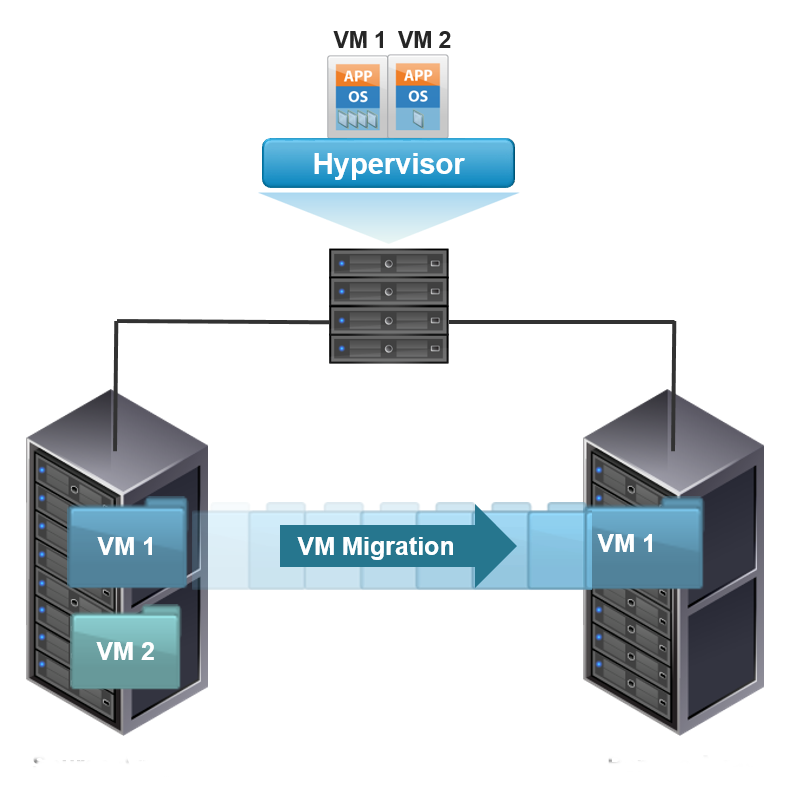
\includegraphics[width=300px]{img/vms_migration.eps}
 \caption{Live migration}
 Fonte: \citet{spaniol2015}
 \label{fig:vms_migration}
\end{figure}

Neste capítulo, durante a escolha das ferramentas, foi efetuado alguns testes experimentais para melhor entender e avaliar as ferramentas, 
sendo que esses testes foram apenas para entendimento. Assim possibilitando escolha mais adequada para o ambiente da empresa.

% Corosync provides pacemaker:
% a mechanism to reliably send messages between nodes,
% notifications when machines appear and disappear
% a list of machines that are up that is consistent throughout the cluster 
% Heartbeat provides:
% a mechanism to reliably send messages between nodes,
% notifications when machines appear and disappear
% a list of machines that are up that is consistent throughout the cluster 
% --
% http://serverfault.com/questions/269831/relation-between-heartbeat-openais-corosync
% well i reached answer on myself! clustering include two part:
% 1.cluster resource management
% 2.infrastructure with massaging layer
% legacy heartbeat is broken into heartbeat message layer and pacemaker so pacemaker is CRM.
% and we have two option on message layer:heartbeat,openais. openais/corosync is preferred as: http://comments.gmane.org/gmane.linux.highavailability.user/32355
% There are, however, features in Pacemaker that require OpenAIS which will work only with Corosync, not Heartbeat. Those features are concerned 
% with the distributed lock managers used by cLVM (but not regular LVM), GFS/GFS2, and OCFS2. If you need that functionality, you must select 
% OpenAIS/Corosync. If you do not, you're free to choose.
% as: http://www.clusterlabs.org/wiki/FAQ
% Originally Corosync and OpenAIS were the same thing. Then they split into two parts... the core messaging and membership capabilities are now 
% called Corosync, and OpenAIS retained the layer containing the implementation of the AIS standard.
% Pacemaker itself only needs the Corosync piece in order to function, however some of the applications it can manage (such as OCFS2 and GFS2) 
% require the OpenAIS layer as well.
% so i went to openais/corosync and integrate it with pacemaker.
% --
% There are, however, features in Pacemaker that require OpenAIS which
% will work only with Corosync, not Heartbeat. Those features are
% concerned with the distributed lock managers used by cLVM (but not
% regular LVM), GFS/GFS2, and OCFS2. If you need that functionality, you
% must select OpenAIS/Corosync.
% 
% Pacemaker itself only needs the Corosync piece in order to function, however some of the applications it can manage 
% (such as OCFS2 and GFS2) require the OpenAIS layer as well. 
